\section{Evaluation}
\label{sec:eval}

The evaluation is a progressive falsification of existing gate designs (RQ1--RQ3), followed by validation of the structured gate's orthogonal properties---containment under attack (RQ4) and generalization (RQ5). \textbf{RQ1}: does a binary terminal gate deadlock multi-step post-violation recovery? \textbf{RQ2}: does scalar admission, swept up to $20\%$ slack, close the gap to structured admission? \textbf{RQ3}: does the predicted projection-trap plateau signature appear, and is it gate-induced rather than reflecting an unrecoverable underlying state? \textbf{RQ4}: under LLM-side compromise (prompt injection, observation poisoning, stall, and magnitude redistribution), does the verifier prevent system worsening and false recovery? \textbf{RQ5}: does the terminal-versus-structured dichotomy generalize across model families and a second domain?

\subsection{Setup}
\label{sec:eval:setup}

We use Gym-ANM ANM6-Easy~\cite{henry2021gymanm} as the critical-infrastructure simulator, integrated as a \silr{} domain with a deep-copy shadow manager and a Newton--Raphson power-flow solver that is bit-exact across repeated solves ($\sigma{=}0$ over $100$ trials). The LLM is Qwen3-14B~\cite{qwen3} served via vLLM at temperature $0$. Each ReAct episode runs with $C_{\text{step}}{=}8$ control steps and $C_{\text{prop}}{=}3$ per-step proposals.

\paragraph{Scenarios.}
We mine a 600-scenario pool by gridded perturbation of load/generation multipliers, source seed, and storage SoC, classified by recoverability (\emph{single-action} 153, \emph{multi-action} 24, \emph{MPC-residual} 252, trivial 171). The multi-action band---$8$ operating points $\times\,3$ storage-SoC perturbations---is our benchmark; each scenario is MPC-recoverable (gym-anm \texttt{MPCAgentConstant} oracle), so the comparison is well-posed. The matched deep contrast (RQ1--RQ3) uses three operating points at $N{=}7$, denoted \texttt{multi\_1}--\texttt{multi\_3} (seeds $1003$--$1009$, $21$ episodes each, $C_{\text{step}}{=}8$); to rule out scenario selection we additionally evaluate \emph{all $24$} at $N{=}5$. Generalization and security suites use $N{=}5$.

\paragraph{Policies.}
\texttt{OFF} (no verifier; every proposal applied), \texttt{terminal} (terminal predicate: admit iff $S(\hat{s}_{t+1})=\emptyset$), \texttt{progress} ($\psione\wedge\psitwo$), \texttt{progress\_mag} ($\psione\wedge\psitwo\wedge\psithree$; the structured admission gate). For the scalar falsifier we add \texttt{scalar\_progress}$_\eta$, admitting iff $P(\hat{s}_{t+1})\le(1{+}\eta)P(s_t)$ with $\eta\in\{0,0.05,0.10,0.20\}$.

\subsection{RQ1: Binary Terminal Admission Deadlocks Multi-Step Recovery}
\label{sec:eval:rq1}

Table~\ref{tab:rq1} reports the headline result at \emph{matched} $N{=}7$ under $C_{\text{step}}{=}8$. Terminal recovers $0/21$ (reject/prop $1.000$): it rejects every intermediate proposal because $S(\hat{s}_{t+1})\ne\emptyset$ at every proposed step, regardless of search depth. Structured admission recovers $\mathbf{21/21}$ (CI $[0.85, 1.00]$, residual $0.000$), while the scalar sweep peak ($9/21$) has a CI disjoint from it---the scalar gap is not sampling noise.

\begin{table}[tb]
\centering
\caption{RQ1: mined multi-action recovery at matched $N{=}7$ ($21$ episodes/policy, $C_{\text{step}}{=}8$). Scalar row = sweep peak ($\eta{=}0.05$); Wilson 95\% CI. Material worsening is $0/21$ for every gated policy; ungated \texttt{OFF} worsens $12/21$.}
\label{tab:rq1}
\footnotesize
\begin{tabular*}{\textwidth}{@{\extracolsep{\fill}}lcccc}
\toprule
Policy & Recovery & 95\% CI & \makecell{Final pen.\\(mean)} & \makecell{Reject /\\prop.} \\
\midrule
\texttt{OFF} (no gate)                      & $1/21$   & $[0.01,0.23]$ & $15.594$ & $0.000$ \\
\texttt{terminal}                           & $0/21$   & $[0.00,0.15]$ & $12.451$ & $1.000$ \\
\texttt{scalar\_progress} (sweep peak)      & $9/21$   & $[0.24,0.63]$ & $4.950$  & $0.408$ \\
\texttt{progress}                           & $20/21$  & $[0.77,0.99]$ & $0.195$  & $0.336$ \\
\texttt{progress\_mag}                      & $\mathbf{21/21}$ & $\mathbf{[0.85,1.00]}$ & $\mathbf{0.000}$ & $0.316$ \\
\bottomrule
\end{tabular*}
\end{table}

The terminal deadlock is structural---the gate refuses every intermediate proposal regardless of search depth---and the lift over the scalar peak ($9/21$) is structural too: support admission alone closes most of it (RQ2).

\subsection{RQ2: Scalar Admission Is Insufficient---A Threshold Sweep Falsifier}
\label{sec:eval:rq2}

If the binary terminal gate fails only because it is too strict, the natural fix is to admit any proposal whose aggregate penalty $P$ is non-increasing or within a small slack of $P(s_t)$. We test this directly with the \texttt{scalar\_progress} family, sweeping the relative slack $\eta$ from strict ($0$) to $20\%$ at matched $N{=}7$ ($21$ episodes/setting, $C_{\text{step}}{=}8$).

Relaxing the threshold neither closes the gap nor improves monotonically: across $\eta\in\{0,0.05,0.10,0.20\}$ recovery is $5/21$, $9/21$, $7/21$, $7/21$, with mean final penalties $4.7/5.0/4.2/2.9$ (default $12.451$) and Wilson 95\% CIs in $[0.11,0.63]$, all disjoint from structured admission's $21/21$ at $[0.85,1.00]$. The non-monotonicity is itself a trap signature: the $\eta{=}0.05\!\to\!0.10$ drop comes entirely from \texttt{multi\_1} ($1\!\to\!0$) and \texttt{multi\_3} ($2\!\to\!0$), while \texttt{multi\_2} rises monotonically to $7/7$. A trace shows the mechanism: on \texttt{multi\_3} (seed $1004$) $\eta{=}0.05$ rejects a step's first two proposals and admits a third, geometry-preserving one to recovery, whereas $\eta{=}0.10$ admits that first proposal and commits to a residual plateau ($P{=}10.86$)---wider slack recovers \emph{less} because admission is a commitment operator (Sec.~\ref{sec:method:trap}). A gate whose recovery rose monotonically in slack would contradict the trap; the non-monotonicity is direct evidence for it.

\paragraph{Structure, not magnitude, drives recovery.}
The lift comes from support geometry, not magnitude: $\psione\wedge\psitwo$ (support inclusion, the $\alpha$-free invariant of Prop.~\ref{prop:inv}) recovers $20/21$ and the full gate $21/21$. Support admission is the recovery driver; the magnitude guard $\psithree$ adds the per-branch protection that RQ4 shows necessary under a redistribution adversary. The gap to scalar is consistent with Prop.~\ref{prop:gap}: it localizes to \texttt{multi\_1}/\texttt{multi\_3}, whose $\preceq$-incomparable geometry no scalar surrogate can order, while \texttt{multi\_2} has no such antichain and every gate clears it. Recovery holds across an $\alpha$-window ($15/15$ for $\alpha\in[1.05,1.20]$, $14/15$ at $\alpha{=}1.02$; $N{=}5$), consistent with the $\alpha$-free support invariant.

\paragraph{The full 24-scenario band.}
To rule out scenario selection, we evaluate all $24$ multi-action scenarios ($8$ operating points $\times\,3$ storage-SoC perturbations) at $N{=}5$ (Table~\ref{tab:band24}). Structured admission recovers the band (\texttt{progress\_mag} $117/120$; \texttt{progress} $116/120$, $\psithree$ again adding a single episode as at the headline), terminal deadlocks, and the scalar gate recovers $101/120$. The band-level scalar gap is real but milder than the headline: smooth operating points and their SoC variants admit scalar descent, so the gap concentrates on the geometry-poor points (RQ3), as the projection mechanism predicts.

\begin{table}[tb]
\centering
\caption{RQ2: full 24-scenario band ($8$ operating points $\times\,3$ SoC perturbations), $N{=}5$, recovery [Wilson 95\% CI]. Structured admission recovers the band; the scalar gap localizes to geometry-poor points; terminal deadlocks.}
\label{tab:band24}
\footnotesize
\begin{tabular*}{\textwidth}{@{\extracolsep{\fill}}lcc}
\toprule
Policy & Recovery & 95\% CI \\
\midrule
\texttt{terminal}                            & $0/120$  & $[0.00,0.03]$ \\
\texttt{scalar\_progress}$_{\eta=0.05}$      & $101/120$ & $[0.77,0.90]$ \\
\texttt{progress}                            & $116/120$ & $[0.92,0.99]$ \\
\texttt{progress\_mag}                       & $\mathbf{117/120}$ & $\mathbf{[0.93,0.99]}$ \\
\bottomrule
\end{tabular*}
\end{table}

\subsection{RQ3: The Scalar Projection Trap---Plateau Signature and Mechanism Validation}
\label{sec:eval:rq3}

The trap (Sec.~\ref{sec:method:trap}) predicts a per-trace signature: the scalar gate accepts one early locally-improving proposal and plateaus while structured admission clears the scenario. It appears across the ordered triple ($N{=}7$, $C_{\text{step}}{=}8$; scalar at its per-scenario \emph{best} $\eta$): \texttt{multi\_2} is smooth (scalar $7/7$ at $\eta{=}0.10$, residual $0.00$); \texttt{multi\_3} plateaus at $\le2/7$ (best $\eta{=}0.05$, residual $5.94$ vs.\ default $17.59$) against structured $7/7$; \texttt{multi\_1} is harder for scalar ($\le1/7$, residual $8.38$ vs.\ default $14.70$) against structured $7/7$. Figure~\ref{fig:trap} contrasts a structured trajectory with the scalar plateau.

\paragraph{The plateau is gate-induced, not an unrecoverable state.}
To confirm the plateau is gate-induced, we hand the scalar-admitted \texttt{multi\_3} plateau to the \texttt{MPCAgentConstant} oracle, which recovers it to zero penalty in one rollout: the structured gate avoids the plateau by declining the geometry-poor first step.

\begin{figure}[tb]
\centering
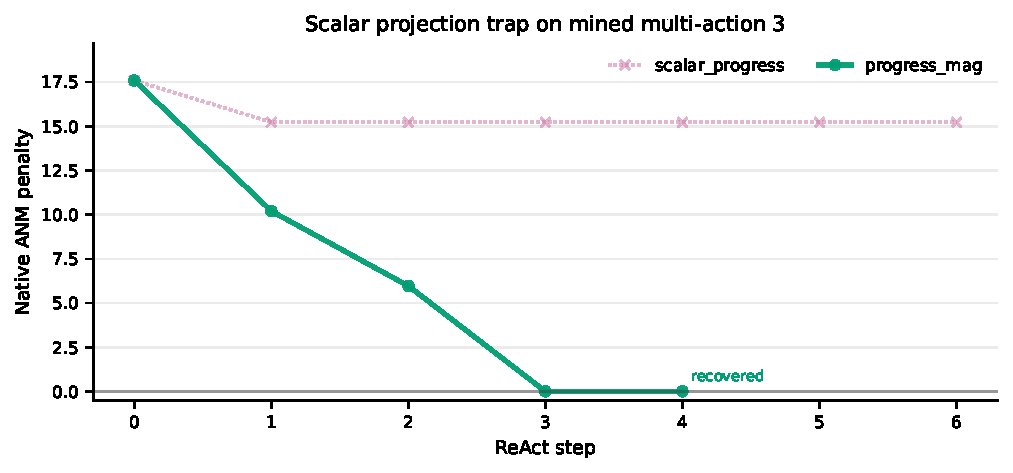
\includegraphics[width=0.44\textwidth]{../figures/mined_multi_action_3_scalar_vs_structured_FINAL.pdf}
\caption{Scalar projection trap on \texttt{multi\_3}. Structured admission (\texttt{progress\_mag}) descends to recovery $\Phi(s){=}(\emptyset,\mathbf{0})$ via accepted \texttt{SAFE\_PROGRESS} steps, whereas the scalar gate admits one early locally-improving proposal and plateaus at nonzero residual across all four slack settings (best $2/7$ at $\eta{=}0.05$).}
\label{fig:trap}
\end{figure}

\subsection{RQ4: Trust-Boundary Containment Under LLM-Side Compromise}
\label{sec:eval:rq4}

The mini-suite runs the three mined multi-action scenarios under \texttt{progress\_mag} with the first three attack families of Sec.~\ref{sec:threat}---prompt injection, observation poisoning, and stall (plain and RAG variants)---at $N{=}5$ per scenario plus a matched benign control: $60$ attack $+\,15$ benign $=75$ episodes, scored by the failure semantics defined there. The fourth family, magnitude redistribution, is evaluated against competing gates below.

Across the $60$ attack episodes the verifier produces $0/60$ attack success, false recovery, and material worsening (Wilson 95\% CI $[0,0.06]$), with $0/15$ on the benign control ($0/75$ overall); under \texttt{prompt\_injection} the rejection rate climbs sharply. Containment is \emph{architectural}, not statistical: the verifier never accesses the LLM's prompt or observation channels (Sec.~\ref{sec:method:shadow}), so any proposal breaching the admission predicates is rejected however the input is corrupted (Prop.~\ref{prop:inv}).

\paragraph{The structured predicate is necessary: magnitude redistribution.}
The fourth family, \emph{magnitude redistribution} (Sec.~\ref{sec:threat}), drives one retained branch toward failure while holding the overloaded-branch set and the aggregate penalty within nominal bounds, evading aggregate- and support-level monitoring. The $39$-episode suite applies this objective across the three scenarios under C1/C2 in three realization variants---direct single-branch concentration, gradual load consolidation, and observation-masked drift (plain and RAG)---all sharing the count-preserving severity signature. A scalar gate is breached $17/39$ and a support-only gate ($\psione\wedge\psitwo$) $12/39$, whereas the full gate ($\psione\wedge\psitwo\wedge\psithree$) is breached $0/39$ (Fig.~\ref{fig:breach}): the aggregate penalty falls and the overloaded-branch \emph{set} is unchanged, so only the per-branch test $\psithree$ rejects the concentrating step.

\begin{figure}[ht]
\centering
\begin{tikzpicture}[font=\sffamily]
  \def\axw{7.2}
  \def\axh{2.7}
  \def\ymax{0.5}
  \pgfmathsetmacro{\sy}{\axh/\ymax}
  \def\bw{1.1}
  \foreach \r in {0,0.1,0.2,0.3,0.4,0.5}{
    \pgfmathsetmacro{\yy}{\r*\sy}
    \draw[gray!22] (0,\yy) -- (\axw,\yy);
    \node[gray!60,font=\scriptsize,left=2pt] at (0,\yy) {\pgfmathprintnumber[fixed,precision=1]{\r}};
  }
  \draw[->,gray!55] (0,0) -- (0,\axh+0.35);
  \draw[gray!55] (0,0) -- (\axw,0);
  \node[gray!70,font=\scriptsize,rotate=90] at (-0.95,\axh/2) {attack breach rate};
  \pgfmathsetmacro{\ha}{0.4359*\sy}
  \fill[oiVermillion] (1.5-\bw/2,0) rectangle (1.5+\bw/2,\ha);
  \node[font=\small\bfseries,above=1pt] at (1.5,\ha) {$17/39$};
  \node[font=\footnotesize,below=3pt] at (1.5,0) {\texttt{scalar}};
  \node[gray!70,font=\scriptsize,below=15pt] at (1.5,0) {aggregate};
  \pgfmathsetmacro{\hb}{0.3077*\sy}
  \fill[oiOrange] (3.6-\bw/2,0) rectangle (3.6+\bw/2,\hb);
  \node[font=\small\bfseries,above=1pt] at (3.6,\hb) {$12/39$};
  \node[font=\footnotesize,below=3pt] at (3.6,0) {\texttt{progress}};
  \node[gray!70,font=\scriptsize,below=15pt] at (3.6,0) {$+$\,support};
  \fill[oiGreen] (5.7-\bw/2,0) rectangle (5.7+\bw/2,0.055);
  \node[font=\small\bfseries,above=2pt,text=oiGreen] at (5.7,0.055) {$0/39$};
  \node[font=\footnotesize,below=3pt] at (5.7,0) {\texttt{progress\_mag}};
  \node[gray!70,font=\scriptsize,below=15pt] at (5.7,0) {$+$\,per-branch};
\end{tikzpicture}
\caption{RQ4: magnitude-redistribution breach rate by admission tier---each added predicate closes more attack surface: scalar $17/39$, support ($\psi_1\wedge\psi_2$) $12/39$, full per-branch ($\psi_1\wedge\psi_2\wedge\psi_3$) $0/39$.}
\label{fig:breach}
\end{figure}

\subsection{RQ5: Generalization Across Families and a Second Domain}
\label{sec:eval:rq5}

The containment result of RQ4 validates the architecture's core invariant; we ask whether the admission-semantics contrast it enables generalizes beyond the primary benchmark.

\paragraph{Cross-family generalization.}
We replicate the terminal-versus-structured contrast across three independent model families---Alibaba Qwen3, Google Gemma-3~\cite{gemma3}, and Meta Llama-3.1~\cite{llama3}---on the same three mined multi-action scenarios at $N{=}5$ (Table~\ref{tab:crossfamily}). The dichotomy is family-independent: terminal deadlocks every model ($0/15$) while structured admission recovers completely ($15/15$ on ANM at $C_{\text{step}}{=}8$), letting compact open-weight models perform the multi-step recovery the terminal gate cannot.

\begin{table}[ht]
\centering
\caption{RQ5: cross-family recovery on the three mined multi-action scenarios, $N{=}5$ (recovery [Wilson 95\% CI]).}
\label{tab:crossfamily}
\footnotesize
\setlength{\tabcolsep}{4pt}
\begin{tabular*}{\textwidth}{@{\extracolsep{\fill}}llccc}
\toprule
Model & Family & terminal & \makecell[c]{\texttt{progress\_mag}\\$C_{\text{step}}{=}8$} & \makecell[c]{\texttt{progress\_mag}\\$C_{\text{step}}{=}16$} \\
\midrule
Qwen3-8B    & Alibaba Qwen3   & $0/15$ & $\mathbf{15/15}$ {\scriptsize[0.80,1.00]} & $15/15$ {\scriptsize[0.80,1.00]} \\
Qwen3-14B   & Alibaba Qwen3   & $0/15$ & $\mathbf{15/15}$ {\scriptsize[0.80,1.00]} & $15/15$ {\scriptsize[0.80,1.00]} \\
Gemma-3-12B & Google Gemma-3  & $0/15$ & $\mathbf{15/15}$ {\scriptsize[0.80,1.00]} & $15/15$ {\scriptsize[0.80,1.00]} \\
Llama-3.1-8B & Meta Llama-3.1 & $0/15$ & $\mathbf{15/15}$ {\scriptsize[0.80,1.00]} & $15/15$ {\scriptsize[0.80,1.00]} \\
\bottomrule
\end{tabular*}
\end{table}

\paragraph{Cross-domain portability.}
We replicate the dichotomy in CityLearn building-energy dispatch~\cite{citylearn} on the same family-spanning subset (Table~\ref{tab:crossdomain}). The three scenarios (\texttt{cl\_1}--\texttt{cl\_3}) instantiate district battery-storage violations (state-of-charge floor/ceiling, feeder-export limits), with $\Phi$ indexed by the violating building or feeder. The gate semantics recur: the terminal predicate clears only the single-step \texttt{cl\_3} ($5/5$) and deadlocks the multi-step \texttt{cl\_1}/\texttt{cl\_2} ($0/10$; the $5/15$ terminal row), while structured admission recovers broadly---$15/15$ for Qwen3-14B and Llama-3.1-8B, $14/15{\to}15/15$ for Qwen3-8B under a doubled budget. Gemma-3-12B reaches $10/15$, its gap confined to \texttt{cl\_2}: the gate admits every Gemma proposal there (all \texttt{SAFE\_PROGRESS}, zero rejections) but its monotone steps stall short of the terminal action stronger models reach. Admission thus ports intact---the gate grades and contains identically---while recovery \emph{completion} remains model-dependent: \emph{structural portability} of the same gate semantics in a distinct physical model.

\begin{table}[ht]
\centering
\caption{RQ5: cross-domain replication on CityLearn (three \texttt{cl} scenarios, $N{=}5$; recovery [Wilson 95\% CI]). \texttt{cl\_3} is single-step recoverable (terminal clears it) while \texttt{cl\_1}/\texttt{cl\_2} are multi-step, mirroring ANM.}
\label{tab:crossdomain}
\footnotesize
\setlength{\tabcolsep}{5pt}
\begin{tabular*}{\textwidth}{@{\extracolsep{\fill}}lccc}
\toprule
Model & terminal & \texttt{progress\_mag} step~$8$ & \texttt{progress\_mag} step~$16$ \\
\midrule
Qwen3-14B    & $5/15$ {\scriptsize[0.15,0.58]}  & $\mathbf{15/15}$ {\scriptsize[0.80,1.00]} & --- \\
Qwen3-8B     & $5/15$ {\scriptsize[0.15,0.58]}  & $14/15$ {\scriptsize[0.70,0.99]} & $\mathbf{15/15}$ {\scriptsize[0.80,1.00]} \\
Gemma-3-12B  & $5/15$ {\scriptsize[0.15,0.58]}  & $10/15$ {\scriptsize[0.42,0.85]} & $10/15$ {\scriptsize[0.42,0.85]} \\
Llama-3.1-8B & $5/15$ {\scriptsize[0.15,0.58]}  & $\mathbf{15/15}$ {\scriptsize[0.80,1.00]} & --- \\
\bottomrule
\end{tabular*}
\end{table}

\subsection{Verifier Overhead}
\label{sec:eval:cost}

Each verifier call performs one $\mathrm{copy}\to\mathrm{apply}\to\mathrm{solve}$ plus three predicate evaluations: $17.5$--$30.0$\,ms on one CPU core, dominated by the solver---under $0.15\%$ of the $\sim$22\,s wall-clock of one LLM ReAct step.
